% f-dnn-architecture — DNN (MLP) architecture, after Lago et al. (2021), Fig. 4.
% Standalone TikZ figure: compile with pdflatex/lualatex. Caption lives in the chapter.
\documentclass[tikz,border=6pt]{standalone}
\usetikzlibrary{positioning, arrows.meta, fit, calc, backgrounds}

\begin{document}
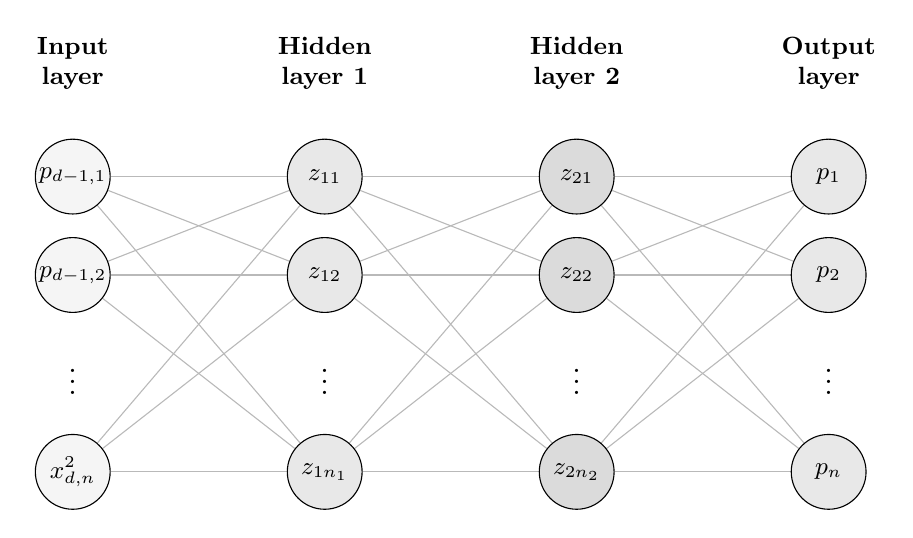
\begin{tikzpicture}[
  >={Stealth[length=5pt]},
  neuron/.style={circle, draw, minimum size=0.95cm, font=\small, inner sep=0pt},
  inlayer/.style={neuron, fill=gray!8},
  h1layer/.style={neuron, fill=gray!18},
  h2layer/.style={neuron, fill=gray!28},
  outlayer/.style={neuron, fill=gray!18},
  dots/.style={font=\large},
  conn/.style={draw=gray!55, line width=0.4pt},
  ltitle/.style={font=\small\bfseries, align=center},
]

% layer x-positions
\def\xa{0}  \def\xb{3.2}  \def\xc{6.4}  \def\xd{9.6}
% node y-positions (third row is the vertical-dots marker)
\def\ya{0}  \def\yb{-1.25}  \def\yc{-2.5}  \def\yd{-3.75}

% --- Input layer ---
\node[inlayer] (i1) at (\xa,\ya) {$p_{d-1,1}$};
\node[inlayer] (i2) at (\xa,\yb) {$p_{d-1,2}$};
\node[dots]    (id) at (\xa,\yc) {$\vdots$};
\node[inlayer] (i3) at (\xa,\yd) {$x^{2}_{d,n}$};

% --- Hidden layer 1 ---
\node[h1layer] (a1) at (\xb,\ya) {$z_{11}$};
\node[h1layer] (a2) at (\xb,\yb) {$z_{12}$};
\node[dots]    (ad) at (\xb,\yc) {$\vdots$};
\node[h1layer] (a3) at (\xb,\yd) {$z_{1n_1}$};

% --- Hidden layer 2 ---
\node[h2layer] (b1) at (\xc,\ya) {$z_{21}$};
\node[h2layer] (b2) at (\xc,\yb) {$z_{22}$};
\node[dots]    (bd) at (\xc,\yc) {$\vdots$};
\node[h2layer] (b3) at (\xc,\yd) {$z_{2n_2}$};

% --- Output layer ---
\node[outlayer] (o1) at (\xd,\ya) {$p_{1}$};
\node[outlayer] (o2) at (\xd,\yb) {$p_{2}$};
\node[dots]     (od) at (\xd,\yc) {$\vdots$};
\node[outlayer] (o3) at (\xd,\yd) {$p_{n}$};

% --- fully-connected edges (real nodes only), drawn behind the neurons ---
\begin{scope}[on background layer]
  \foreach \s in {i1,i2,i3}{\foreach \t in {a1,a2,a3}{\draw[conn] (\s) -- (\t);}}
  \foreach \s in {a1,a2,a3}{\foreach \t in {b1,b2,b3}{\draw[conn] (\s) -- (\t);}}
  \foreach \s in {b1,b2,b3}{\foreach \t in {o1,o2,o3}{\draw[conn] (\s) -- (\t);}}
\end{scope}

% --- layer titles ---
\node[ltitle, above=0.5cm of i1] {Input\\layer};
\node[ltitle, above=0.5cm of a1] {Hidden\\layer 1};
\node[ltitle, above=0.5cm of b1] {Hidden\\layer 2};
\node[ltitle, above=0.5cm of o1] {Output\\layer};

\end{tikzpicture}
\end{document}
